\documentclass{article}
\usepackage{graphicx}
\usepackage{amsmath}
\usepackage[parfill]{parskip}
\usepackage{hyperref}
\usepackage{appendix}
\usepackage[l3]{csvsimple}
\usepackage{glossaries}
\usepackage{tabularx}
\graphicspath{ {./figures/} }

% reference-managing package
\usepackage{biblatex}
\addbibresource{references.bib}

\title{Quantitive study on the Database marketplace}
\author{Cuong Nguyen}
\date{22/04/2022}

\makeglossaries{}
\loadglsentries{tex/glossary.tex}


\begin{document}
    
\maketitle

\tableofcontents

\printglossary{}

\section{Abstract}\label{sec:abstract}
In this report, I aim to study the detail numerical statistic of Database marketplace,
which are price range, mean, median price of each type of products and all items in
the whole dataset. Given a JSON dataset, scrapping and crawling the whole marketplace website
by Juha Nurmi and others, I developed and extracted more key fields which are
very informative in grouping product types and generating statistical results.
Based on the analytical results, I observe that the average price of products
traded in Database marketplace is not very high, affordable for most of buyers.
In addition, personal information and banking/credit data are widely sold on
the dark marketplace. Those sensitive data is highly possible leaked from major
data breaches. Without raising the awareness of securing personal data,
more people will suffer increasingly financial and mental damage.
\pagebreak

\section{Background}\label{sec:background}
In this section, I will describe theoretical concepts: Tor network, Onion service,
Cryptocurrency, Dark marketplace.

% Tor network
\subsection{Tor network}
Tor is the second generation of onion routing system that addresses shortcomings
in the original design by adding perfect forward secrecy, congestion control,
directory servers, integrity checking, configurable exit policies, and a
practical design for location-hidden services through rendzvous points
~\cite{paper:tor_design}. Tor is a low-latency network system, which means that
the period of delaying is negligible for most users~\cite{report:overview_tor}.
This advantage makes Tor as a
suitable design for interactive tasks like web browsing or \acrshort{ssh}
connections~\cite{dis:usage_of_onion_services}. In addtion to the fast performance,
Tor communication service also provides the high degree of anonymity and privacy
in transferring network packets. Hence, Tor browser, a Firefox-based web browser
under Tor network, is widely used by activists and journalists for untraceable
communication~\cite{dis:usage_of_onion_services}. Moreover, ordinary citizens who have concerned their privacy during
Internet surfing select Tor-based applications as safe guards in the ungovernable
Internet environment.

The Tor users are protected by the common method of Internet surveillance, traffic
analysis. The source and destination of Internet communication can be exposed by
traffic analysis. These information reveal users' behaviour and interest~\cite{web:onion_network}.
To reduce the risk of traffic analysis, Tor distribute the connection between the
client and the final point over the chain of 3 Tor nodes, called \emph{relays}.
The circuit of encrypted connection over relays is described as the following steps.
% How does Tor anonymously route packets
\begin{enumerate}
    \item The Tor user obtains a list of Tor nodes from a
    directory server. Then public keys of selected relays are used to encrypt and
    encapsulate the network packet.  
    \item The Tor client connects to the guard relay, the first relay in the circuit
    of three Tor nodes. The encapsulated message is delivered to the guard relay.
    \item The guard relay decrypts the packet, using its private key, 
    and forward to the second node, the middle relay.
    \item The second node continues decrypting, using its private key, and then
    forwarding the message to the third node, the exit relay.
    \item The exit relay decrypts, using its private key, and forward the packet
    to the final destination, e.g, a web server.
\end{enumerate}

As shown in the aforementioned steps, a specific Tor relay only knows about the previous
sender and the next recipient. For example, the guard relay only learns about the Tor client
and the second hop, but not the final recipient. Thus, a complete path from the original
sender to the final destination is not exposed.

At each hop, the packet is decapsulated and decrypted by using private key of each relay,
``peeling off'' each encryption layer. It is similar to layers of onion and that is also
the reason why it is called \emph{onion routing}.

Although the traffic correlation attack is unavoidable in any low-latency anonymity
network, it is challenging to perform global traffic analysis due to the huge amount
of Tor users~\cite{dis:anonymity_system,paper:tor_design}. In addition to traffic and
time analysis, there are other techniques that reveal real identity of Tor users
~\cite{paper:de_tor}.

There are several types of routers, or relays, in the Tor network and soem of them
are aforementioned, including guard, middle, and exit. Since the exit relay communicates
publicly, outside the Tor network, to the destination, the IP address of it is exposed.
Moreover, the sender can also know the IP address of the first relay in the circuit of
three Tor routers.
By blocklisting the IP addresses of theses publicly known relays, many governments block
connections from their citizens to the Tor network. To address this problem, the bridge
node which is not listed in the public Tor directory is introduced. Thus, it is difficult
to block an IP address if it is not publicly known. However, several countries have
found means to detect and block connections to Tor bridges. Pluggable transport, a
special kind of bridge, is discovered address this problem by adding an extra layer
of obfuscation~\cite{web:relay_types}. According to \url{https://metrics.torproject.org},
in 2021, there are around 7000 relays and more than 2000 bridges running in the Tor
network.

Tor enables TCP-based applications to acquire online anonymity without modification
~\cite{paper:tor_design}. One of the popular Tor application is Tor browser. It is
a modified version of Mozilla Firefox Extended Support Release (ESR) with most-strict
security settings, such as NoScript and HTTPS Everywhere. This browser routes all
traffic through the Tor network and removes all possible fingerprinting methods,
including forging information about the operating system and hardwares
~\cite{dis:usage_of_onion_services}.
Furthermore, Tor Browser does not save sensitive data, including browsing history,
cache and cookies~\cite{dis:usage_of_onion_services}.

% Onion services
\subsection{Onion service}
%
Onion services, Tor hidden services, are an overlay network on top of TCP/IP;
thus, IP addresses are not used in the protocol~\cite{web:onion_service}. The
location and real IP address of Onion Service are protected, hidden from the
user. These hidden services are only available through the Tor network~\cite{paper:tor_design}.
Instead of IP address, onion service is indentified by the \emph{identity public key}.
This onion address which is in the form of \emph{x.onion} whose the first part \emph{x} is
the hash of public key of onion service, e.g, {\scriptsize \textbf{
database6e2t4yvdsrbw3qq6votzyfzspaso7sjga2tchx6tov23nsid.onion}}~\cite{dis:usage_of_onion_services}.

The onion service hides and protects itself by only allowing direct connections
from three pre-selected Tor relays, \emph{introduction points}. Every Tor client
and intermediary points have to be introduced by the three-hop circuit to reach
the onion service.
To be noticeable to clients, instead of using \gls{dns}, \gls{dht} is utilized
to match a onion service to its corresponding introduction points.

The onion service protocol is summarized in the following steps~\cite{paper:tor_design}.
\begin{enumerate}
    \item The onion service selects three Tor relays acting as its introduction
    points to build an anonymized circuit.
    \item The onion service generates a \emph{descriptor}, containing a list of
    introduction points, and signs this descriptor with the \emph{identity private
    key}. The key used to signing is the private part of the identity public key
    which is encoded in the onion service address.
    \item Given the onion address, the client requests the signed descriptor from
    from the \acrshort{dht}. Next, the client verify the signature of returned
    descriptor with the public key that is encoded in the onion address.
    \item The client randomly selects a Tor relay acting as a rendezvous point,
    build anonymized, three-hop circuit to it and send it an one-time secret.
    \item The generated one-time secret and the address of the rendezvous point
    are encrypted with the public key of the onion service and delivered to one of
    the introduction points through a anonymized circuit.
    \item The onion service decrypts and retrieve the rendezvous point and one-time
    secret. It connects and sends the one-time secret to the rendezvous point via
    a three-hop circuit.
    \item A complete circuit between the client and the onion service is built.
    It contains total five Tor relays, two from the client to the rendezvous point
    and three from the rendezvous point to the onion service. 
\end{enumerate}

The onion service protocol provides both end-to-end encryption and authentication
~\cite{web:onion_service}. Hence, it is impossible to censor onion services
and \gls{mitm} attack is prevented~\cite{dis:usage_of_onion_services}. As onion service
can publish contents anonymously, some of them are the sources of adverse content,
including illegal traded products, images of child abusing, etc~\cite{dis:usage_of_onion_services}.
However, many onion services
share content supporting human rights, meaningful for journalism and publishing
content that is censored by oppressive governments~\cite{dis:usage_of_onion_services}. 

\begin{figure}
    \centering
    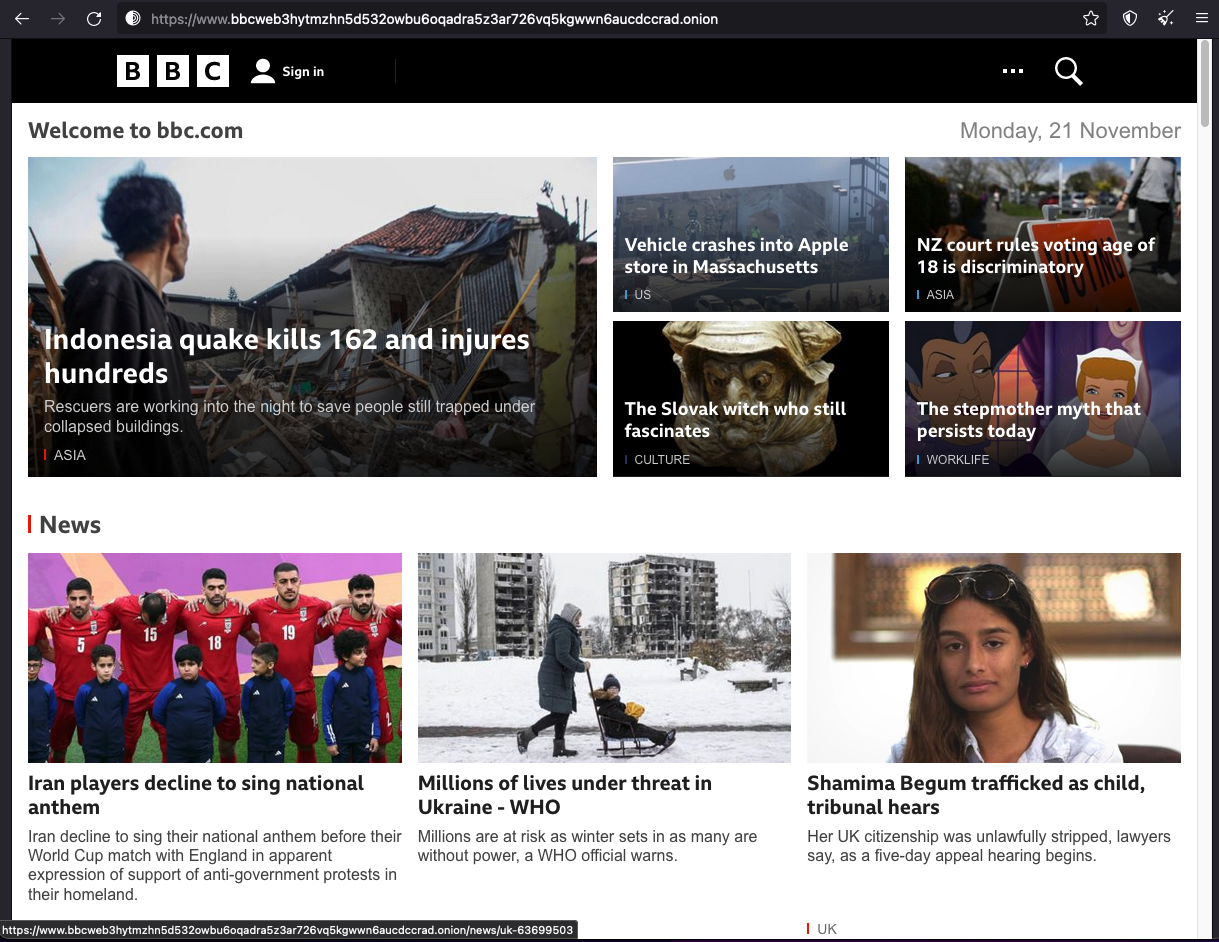
\includegraphics[width=\textwidth,height=\textheight,keepaspectratio]
    {screenshots/bbc_onion.png}
    \caption{Onion service mirroring BBC news website on Tor network.}
    \label{fig:onion_service}
\end{figure}

% Monetary system
\subsection{Cryptocurrency}
%
Onion service provides location hiding capacity and anonymity in content publishing
for illegal markeplaces. However, they also need a payment system that is untraceable and secure,
which is impossible to know exactly involving parties. Hence, the creation of pseudonymous
unregulated electronic money leads to the increasing number of illegal marketplaces
is formed~\cite{dis:usage_of_onion_services}.

In 2009, someone who has pseudo name Satoshi Nakamoto created the peer-to-peer digital
cash system~\cite{misc:bitcoin_origin}. This electronic money, widely known as Bitcoin,
is the first distributed digital currency that works without a trusted third party
~\cite{dis:usage_of_onion_services,misc:bitcoin_origin}. Bitcoin operates based on
cryptographic proof instead of trust, trading directly between users~\cite{misc:bitcoin_origin}.
Several security mechanism, including hash checksums and proof-of-work, are implemented
to protect users from transaction spoofing~\cite{dis:usage_of_onion_services}.

The amount of bitcoins is limited, 21 million bitcoins; thus, its price depends on
the continuos demand to exchange this currency among its netowrk or to other
currencies~\cite{misc:bitcoin_origin,dis:usage_of_onion_services,paper:bitcoin_finance}.

Although Bitcoin system does not provide high degree of technical anonymity, it is
widely used as the main method of payment in illegal commerce website hosted in
the Tor network~\cite{dis:usage_of_onion_services}. In addition to Bitcoin, there
are several cryptocurrencies, including Monero, Zcash, Litecoin, etc., that are
utilized for trading in Tor-based marketplaces.

% Black markeplace
\subsection{Dark marketplace}
%
Silk Road, a dark marketplace, is an ideal case to study the impact of anonymous
online communication on the transformation of crime, from offline to online
environment~\cite{paper:ebay_drugs_22}. With the support of identity-hidden
services, illegal trade is significantly expanded. There are two essential
components of a dark marketplace~\cite{dis:usage_of_onion_services}:

\begin{enumerate}
    \item A network that provides high degree of anonymity whose the market website
    is hosted.
    \item A payment system that is not only secure but also exhaustively to trace
    involving parties.
\end{enumerate}

Silk Road was the first combination of these components~\cite{dis:usage_of_onion_services}.
In this online market, users --- buyers and sellers --- have their own Bitcoin wallers
~\cite{report:surfing_silk_road_23}.
An \emph{escrow system} that charges a commission fee to the market site and locks
the payment between a buyer and a store~\cite{report:surfing_silk_road_23}. In addition,
a reputation system is introduced to motivate the vendors sell products matching
their advertisements. When a buyer receive a product, if the buyer is happy with
the product, the payment is transferred to the vendor. Otherwise, if the buyer
does not satisfy, the buyer can send a complaint ticket and the market site resolves
the conflict between the buyer and the seller~\cite{report:surfing_silk_road_23}.
The buyer can give feedbacks that is publicly visible for other buyers, making
the reputation system is important for both buyers and sellers~\cite{paper:reputation_sys_79}.

Several academic papers are published researching different sides of Silk Road~\cite{paper:ebay_drugs_22,
report:surfing_silk_road_23,dis:anonymity_system}. It is studied that Silk Road was
a profitable marketplace which trades millions of USD values of illegal drugs per month
~\cite{report:evaluate_Silk_Road_75}.

These kind of black marketplaces operate based on the financial motivation and
the increasing demand of customers. In addition to Silk Road, was shut down in 2013,
there are around 20 different dark marketplaces which are observed huge traffic
~\cite{dis:usage_of_onion_services}. These marketplace can be considered as an
illegal version of Ebay with additional cryptocurrency payment systems, escrow
systems, and reputation systems~\cite{dis:usage_of_onion_services}.

In this study, Database marketplace, also a black marketplace, is examined.
Unlike Silk Road or its variants, whose main products are illegal drugs,
Database market mainly provides personal data --- full name, \acrshort{dob},
\acrshort{ssn}, etc. --- and banking information serving for illicit activities.

\begin{figure}
    \centering
    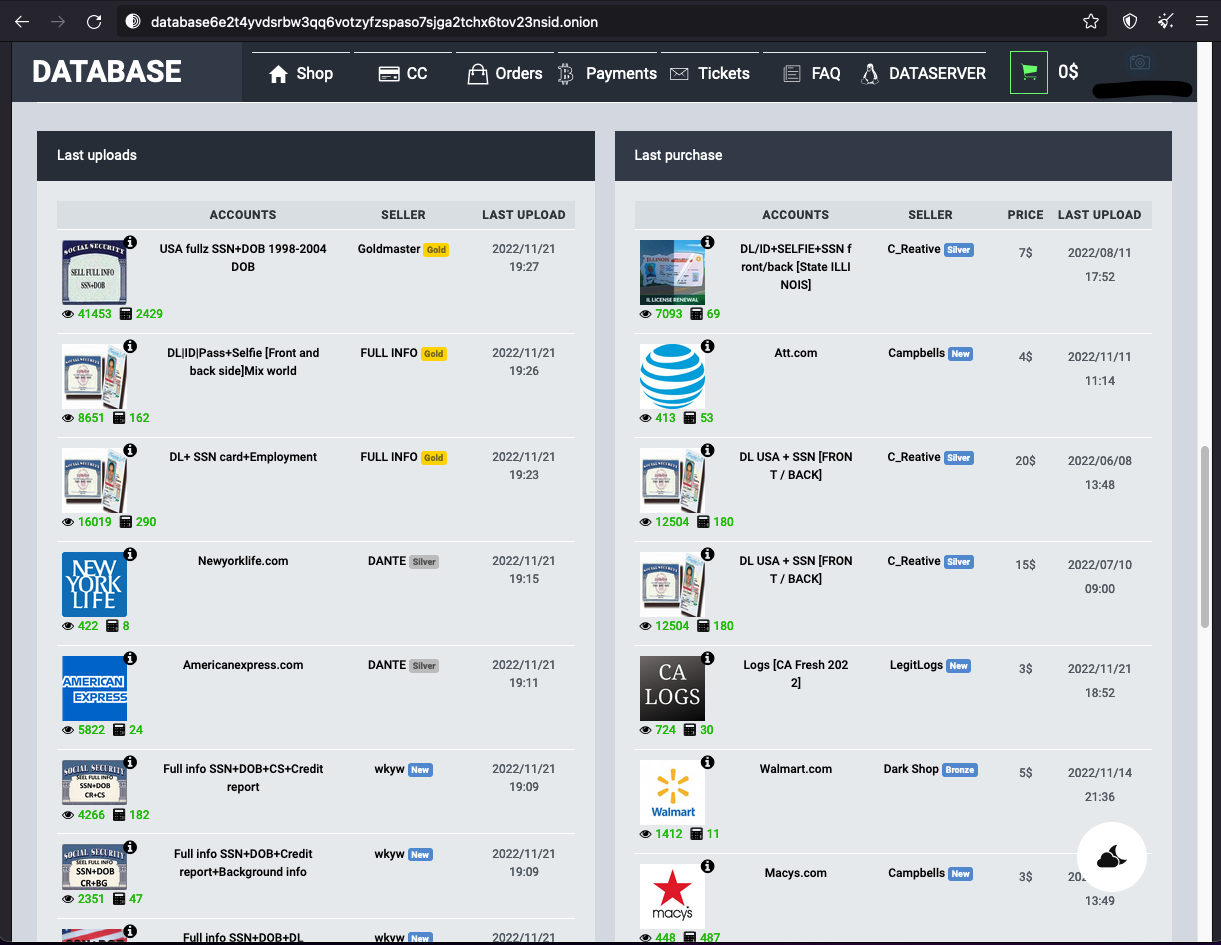
\includegraphics[width=\textwidth,height=\textheight,keepaspectratio]
    {screenshots/database_market_onion_service.png}
    \caption{Homepage of Database marketplace onion service hosted on Tor network.}
    \label{fig:database_homepage}
\end{figure}
\pagebreak

\section{Research questions}\label{sec:research_questions}
Database marketplace sells access to online compromised accounts and other
credential information which can be used for deleterious purposes. For example,
buyers can use sold credit cards to purchase their debts or online items. Another
scenario is that a criminal can utilize personal information to borrow money from
banks, or to make fraudulent health insurance claims\cite{web:personal_info_darkweb}.
Hence, personal data is an attractive item on dark webs, and the breach of it has the
significant impact on society in the financial perspective. In this study, I will
explore the wide range of sensitive data sold on Database marketplace, revealing a
detail picture of stolen personal data sold on the hidden Tor network through the
following research questions:

\begin{enumerate}
    \item What types of stolen information are traded?\label{rq:type}
    \item What are the prices for different product types?\label{rq:price}
    \item Where the stolen information is from?\label{rq:where}
    \item What we can learn about the sellers?\label{rq:seller}
\end{enumerate}
\pagebreak

\section{Methodology}\label{sec:method}
\subsection{Research design}
In order to answer research questions, I explored more key fields from the initial
database. These fields includes price, date, product type, and shop information.
By applying appropriate statistic on key fields, I produced conclusions based on
numerical results. In addtion, manually discovering the Database market, I captured
a certain of screenshots that support my observation.

In order to replicate my result, please do the following steps:

\begin{enumerate}
    \item Access the original dataset provided by Juha Nurmi at \url{https://
    mega.nz/folder/aJwVyIYJ#}.
    \item Download \emph{database.tar.gz} (7 MB) and follow the instructions
    in \emph{README.md}.
    \item Check \emph{sha256sum}:\\\textbf{5a5f2cb4feb7fee597b0a26b1dc2fb33b1f
    9cae639e995a89663198bcfa76f1a}.
    \item Extract the compressed dataset (tar -xf database.tar.gz).
    \item 33,896 JSON files are generated in the destination folder.
    \item Clone the GitHub repo \url{https://github.com/ancuongnguyen07/Database
    _Market.git} and follow the comprehensive \emph{README.md} document.
\end{enumerate}

%%%%% DATA SAMPLE
\subsection{Samples}
%
The Database Market that sells personal data is accessible through \url{http://d
atabase6e2t4yvdsrbw3qq6votzyfzspaso7sjga2tchx6tov23nsid.onion/} inside the
anonymous Tor network. The initial dataset, provided by teacher Juha Nurmi, can
be downloaded from \url{https://mega.nz/folder/aJwVyIYJ#9SWh-Z3-
TpPfjHZeFxbeew}.
The provided dataset is an archive of 33,896 JSON files, 400 MB of raw size. Each
JSON file is represented as the following fields as shown in \autoref{fig:original_json}:

\begin{itemize}
    \item \emph{url}: URL address of webpage.
    \item \emph{text}: Text of the webpage.
    \item \emph{timestamp}: Data collection date.
\end{itemize}

\begin{figure}
    \centering
    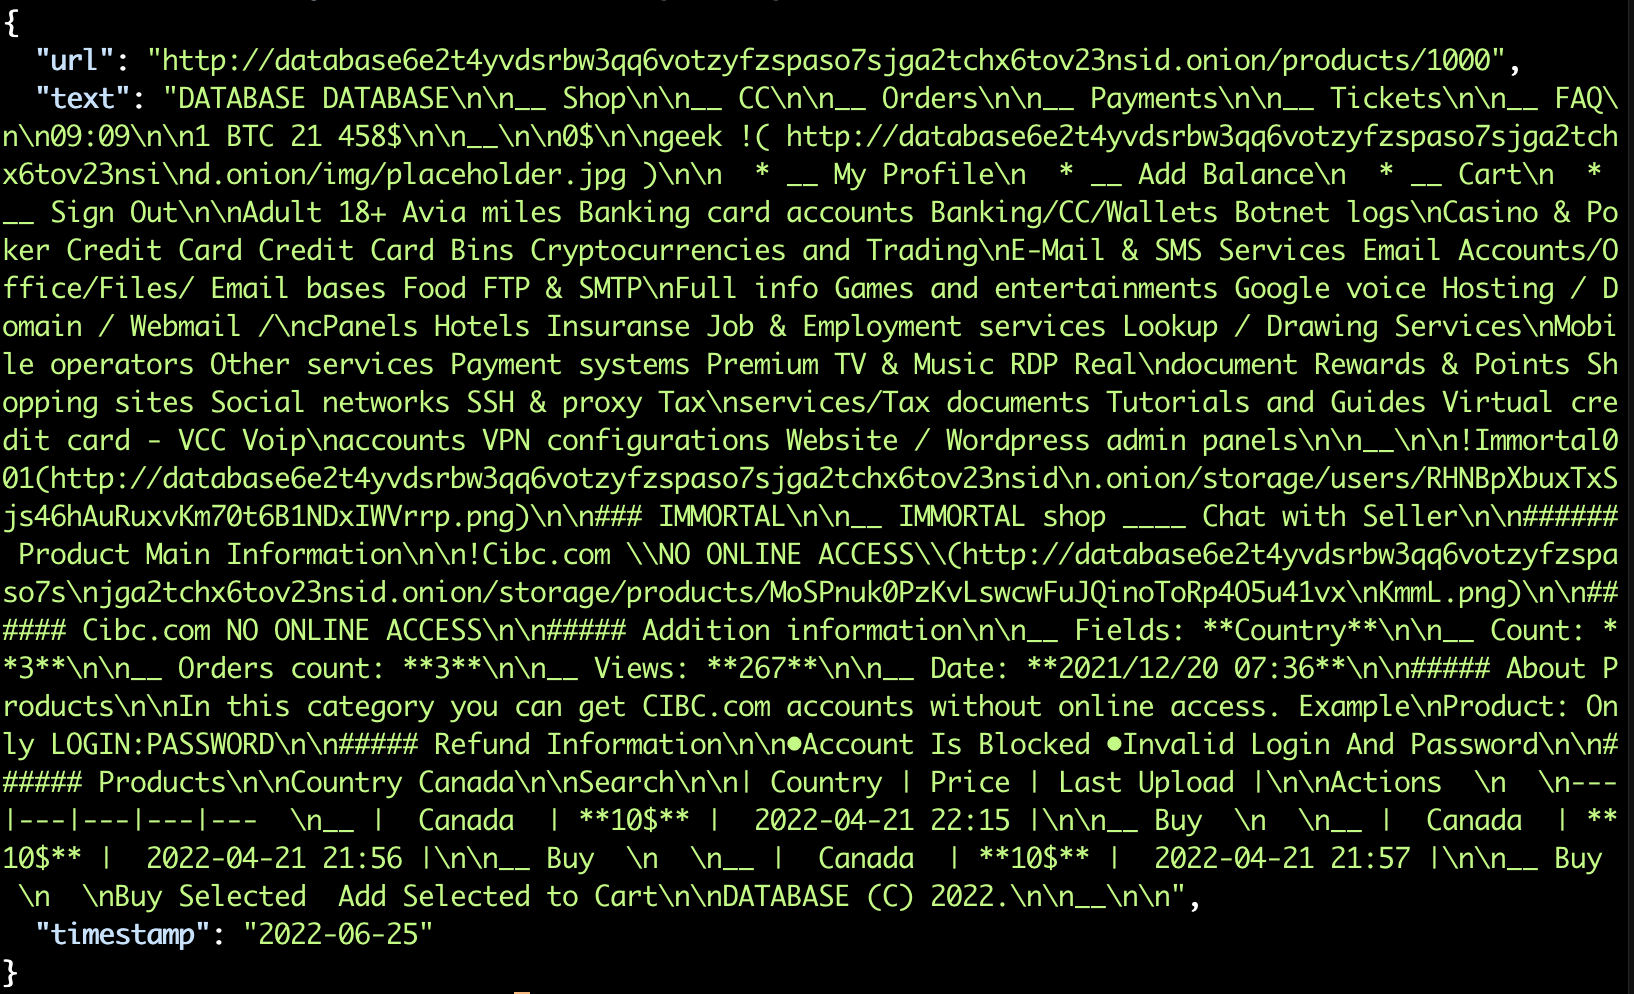
\includegraphics[width=\textwidth,height=\textheight,keepaspectratio]
    {screenshots/orginal_json.png}
    \caption{An example JSON file from the provided dataset by Juha.}\label{fig:original_json}
\end{figure}

In order to achieve more insights of credentials for sale, I produced an additional JSON file
,\emph{ProductPages},that reveals more key features of products sold on a targeted marketplace. Each entry in
the customized JSON file represents a webpage of product containing many sorts of items for sale.
\autoref{fig:custom_json} is an example of an entry, where I assigned the following fields.

\begin{itemize}
    \item \emph{id}: Product ID\@.
    \item \emph{time-stamp}: Data collection date.
    \item \emph{category}: Type of product.
    \item \emph{seller}: Username of seller.
    \item \emph{product}: Name of product.
    \item \emph{prices}: Prices of items.
    \item \emph{dates}: Item uploaded date.
\end{itemize}

\begin{figure}
    \centering
    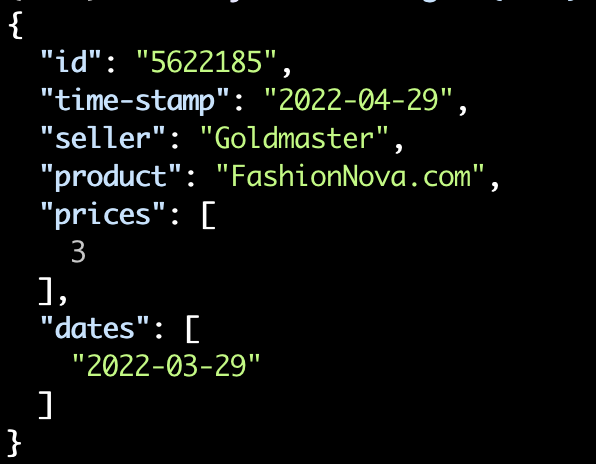
\includegraphics[width=\textwidth,height=\textheight,keepaspectratio]
    {screenshots/customized_json.png}
    \caption{An example JSON entry from my customized dataset}\label{fig:custom_json}
\end{figure}

The datasets are under CC BY 4.0 license: You are free to copy, share, redistribute,
remix, transform, and build upon the material for any purpose, even commercially.
You must give attribution and appropriate credit. Follow the terms: \url{https:/
creativecommons.org/licenses/by/4.0/}.

%%%%% Data collection
\subsection{Data collection}
%
The initial dataset captured web pages of stolen credentials sold in the Database market
from November 2021 to June 2022. Based on that dataset, I extracted a certain of key
fields, including \emph{product, prices, dates} and \emph{seller} for the \emph{text} field.
In addition, I manually took screenshots of pages showing information of products and
stores in Database Market. In order to access a marketplace hosted in Tor network,
it is common that you need an invitation code to register an account on the marketplace.
However, in case of Database Market, I can create an account without an invitation
code.

Filtering interesting fields from the text content in the webpage of product requiring
some marking letters. For example, I noticed that the title of item sold in Database
marketplace is enclosed by ``\#\#\#\#\#\#'', and the store name is covered by ``\#\#\#''. However,
it is more complicated in the cases of \emph{prices} and \emph{dates}. As criminals can
unconstrainedly format the description of their products, I am unable to conduct a common
pattern to capture all prices and dates of uploaded items. Thus, in addition to the quite
effective pattern, returned correct fields in most of pages, I added some criteria for
specific cases. In terms of category, I filtered top common keywords in the title of
products, and grouped items that contain the shared keyword into a category. For example,
any titles containing ``info'', ``ssn'', ``dob'', and ``dl'' belong to the \emph{Personal
data} category.

%%%% Data analysis
\subsection{Data analysis}
%
Applying statistic to the whole dataset, \emph{ProductPages}, I obtained the following
numerical results shown in \autoref{tab:dataset_stat}.

\begin{table}
    \centering
    \begin{tabular}{|c|c|}
        \hline
        Total number of items & 53815\\
        Total number of stores & 30\\
        Maximum price & 2500.00 USD\\
        Minimum price & 0.20 USD\\
        Average price & 15.87 USD\\
        Median price & 5.00 USD\\
        \hline
    \end{tabular}
    \caption{Statistical result of the \emph{ProductPages} dataset.}
    \label{tab:dataset_stat}
\end{table}

The maximum 2500 USD, or other prices greater than 1000 USD, appears with a low
frequency, an outlier. In this case, 2500 USD is a price of a set of 1000 personal data
entries. On the other hand, the average price of personal data is 7.73 USD shown
in \autoref{tab:category_stat}. The price of personal data item depends on the amount
of data pieces included. For example, in the product ID 978, 100 USA \acrshort{ssn}+\acrshort{dob}
is sold at 80 USD, while a buyer has to purchase 250 USD to retrieve 500 USA \acrshort{ssn}+\acrshort{dob}.
In addition, the quality of identity information, also influences
the price. For example, in the product ID 5507764, a set of \acrshort{ssn}+\acrshort{dob}+\acrshort{dl}+\acrshort{mmn}
is sold at 5 USD, while a batch of \acrshort{ssn}+\acrshort{dob}+\acrshort{cs} in ID 5434366 is
assigned at 7 USD\@. The quality of identity information here is interpreted as the level
of financial impact and the simplicity to expose other credential data if this
information is compromised.

There are a certain of product types are traded in Database marketplace. However,
two main categories that most of traded items belong to are \emph{Personal data}
and \emph{Online account}, as shown in \autoref{fig:type_allocation}. \emph{Online
account} category contains compromised online accounts from popular services,
including \textit{Netflix}, \textit{Amazon}, \textit{Venmo}, etc. A full list
of attacked websites is accessible via \url{https://github.com/ancuongnguyen07/
Database_Market/blob/main/analysis_result/leaked_websites.txt}.

There are in total 30 stores, or sellers, in the database. \emph{Goldmaster}, the
most active seller, has sold the largest amount of products during 11/2021--06/2022,
11882 items. However, \emph{bussman shop}, a store that has the greatest average price (430 USD),
only sold 9 items. Furthermore, \emph{bussman shop}, provides service of customizing
ID documents for \acrshort{eu}/\acrshort{us}; thus, the prices of it's products are significant
higher than those of other shops, ranging from 80 USD to 1200 USD\@. A table of full
numerical results from analyzing stores is accessible in \url{https://github.com/anc
uongnguyen07/Database_Market/blob/main/analysis_result/seller_stat.csv}.

\begin{figure}
    \centering
    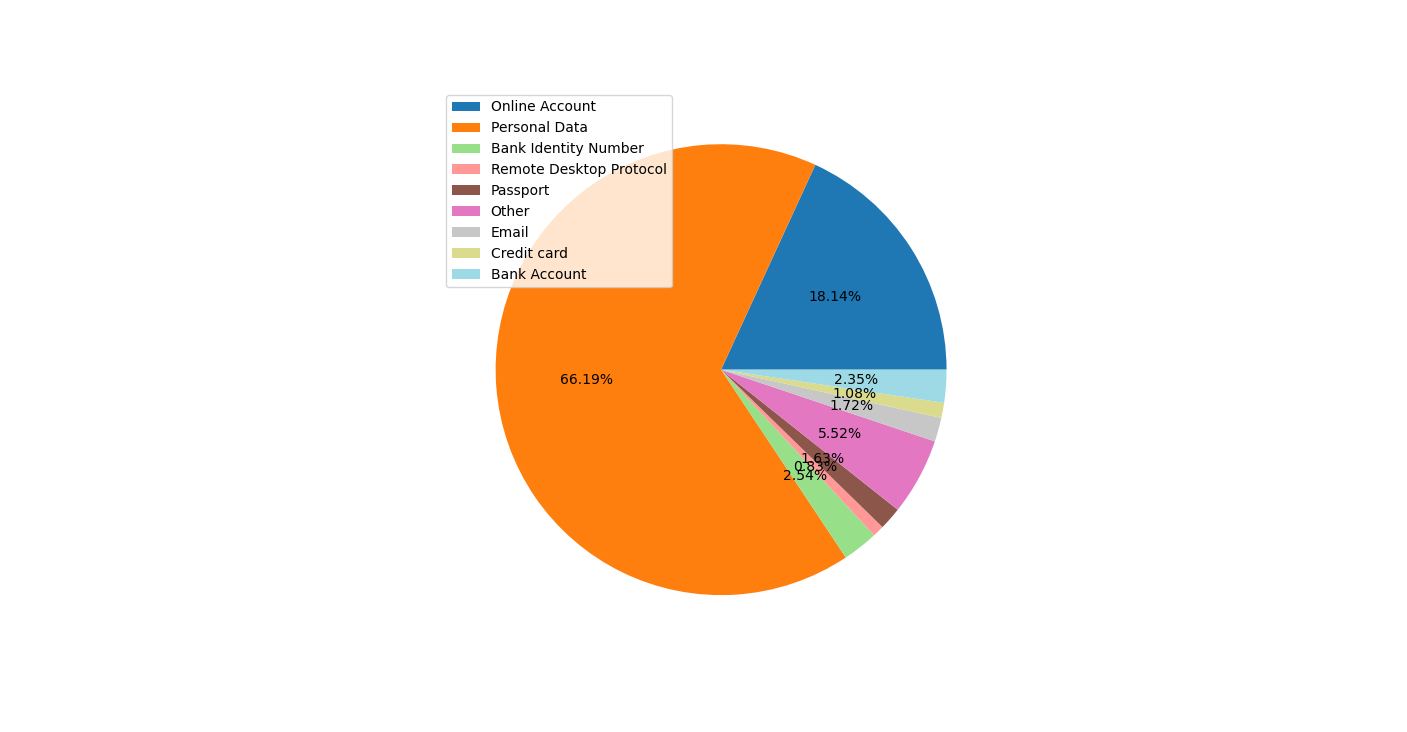
\includegraphics[height=\textheight,width=\textwidth,keepaspectratio]
    {plots/category_allocation.png}
    \caption{Product types allocation.}\label{fig:type_allocation}
\end{figure}

\begin{figure}
    \centering
    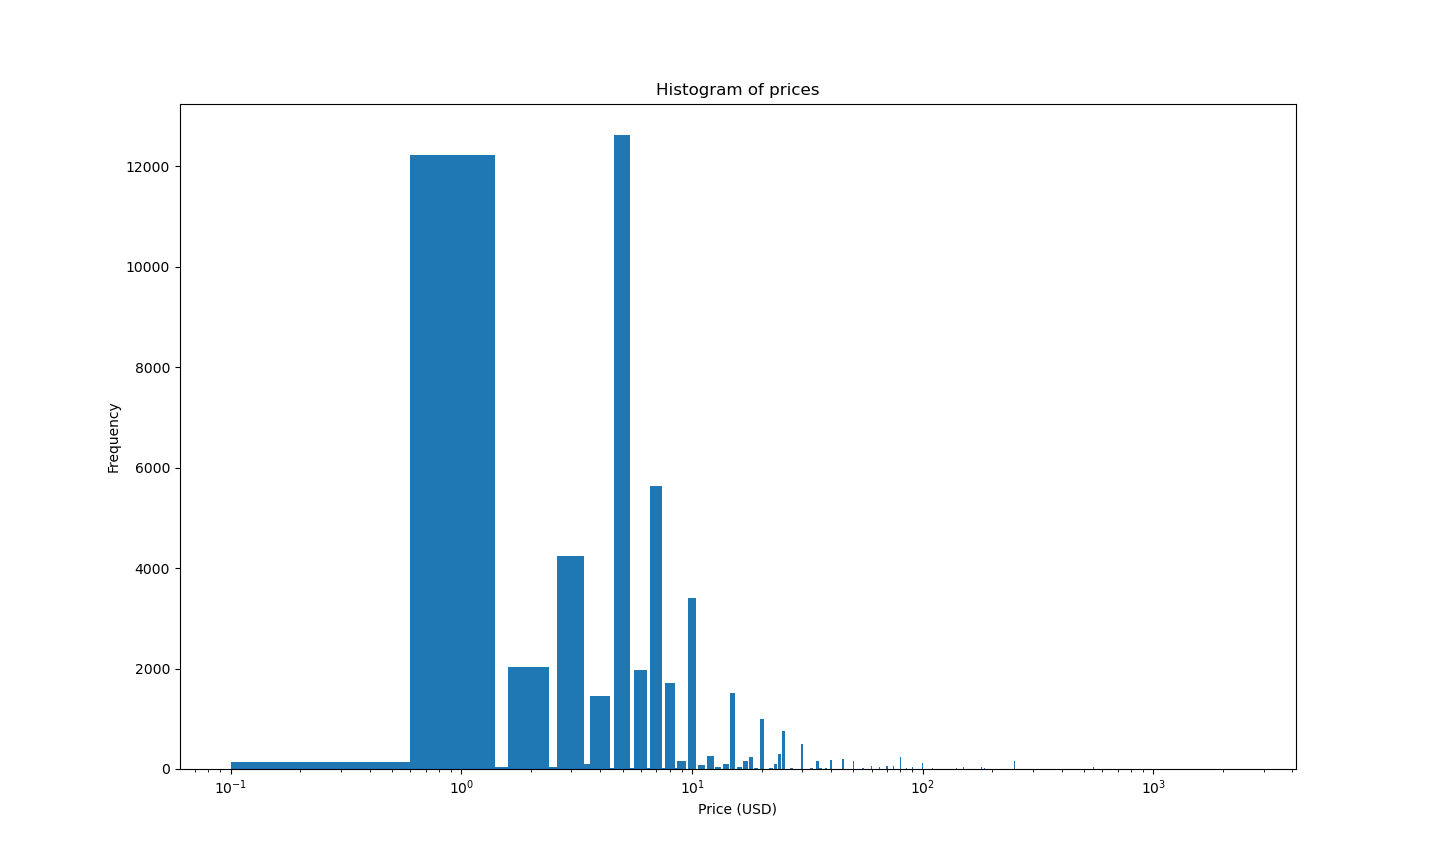
\includegraphics[height=\textheight,width=\textwidth,keepaspectratio]
    {plots/price_histogram.png}
    \caption{Price distribution.}\label{fig:price_range}
\end{figure}

\begin{figure}
    \centering
    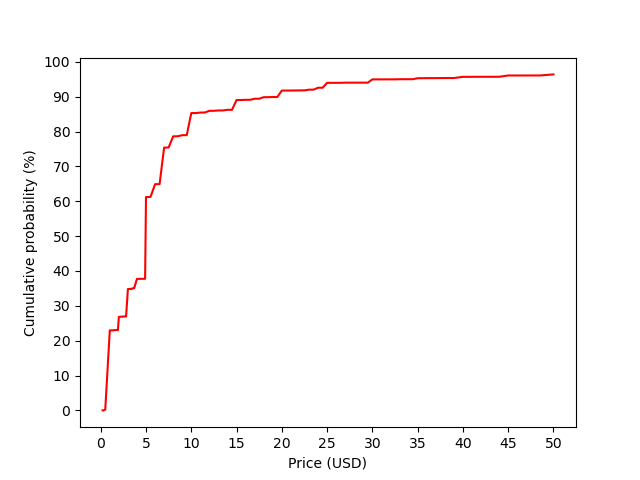
\includegraphics[height=\textheight,width=\textwidth,keepaspectratio]
    {plots/cumprob_price.png}
    \caption{Cumulative probability of price range 0--50 USD.}\label{fig:cum_prob}
\end{figure}

%%%%% Limitation
\subsection{Limitations}
% time range is so far from this moment
The initial database recorded product information in 8 months, from November 2021
to June 2022, covering 33896 product pages. First, the time of writting this study,
November 2022, is 5-month after the last captured product in the database; therefore,
observations and propositions instroduced in this study do not provide the most
updated status of the Database marketplace. In comparison to product entries in
the original database, the marketplace now provides more items; and many products
recorded in the database is now either withdrawed or sold out, i.e product ID
5609797 (\autoref{fig:not_found_prod}).

% seller can freely format product description
In Database marketplace, shops can unconstrainedly format their product description;
thus, I cannot filter exactly interesting fields in all cases, resulting minor noise
in the examination.
% group category manually, by personal preference
Moreover, product category is not provided in the inital database, not even in the
product page. In order to attain product type data, I grouped products that have
the common keywords in a category as presented in \autoref{tab:category_stat}.
This text-based clustering method is not reliable in all cases.

% no feedback information of seller
I examined that there is a shortage of feedback information about stores, or sellers, in
the Database market. As shown in \autoref{fig:seller_asap_market}, in the ASAP marketplace,
feedbacks from customers are classified as negative and positive, that is helpful
to detect an unreliable shop. On the other hand, as presented in \autoref{fig:seller_Database},
Database market does not display feedbacks a specific store, but buyers can send
comments via the internal ticket which is not shown in the store dashboad.

\begin{figure}
    \centering
    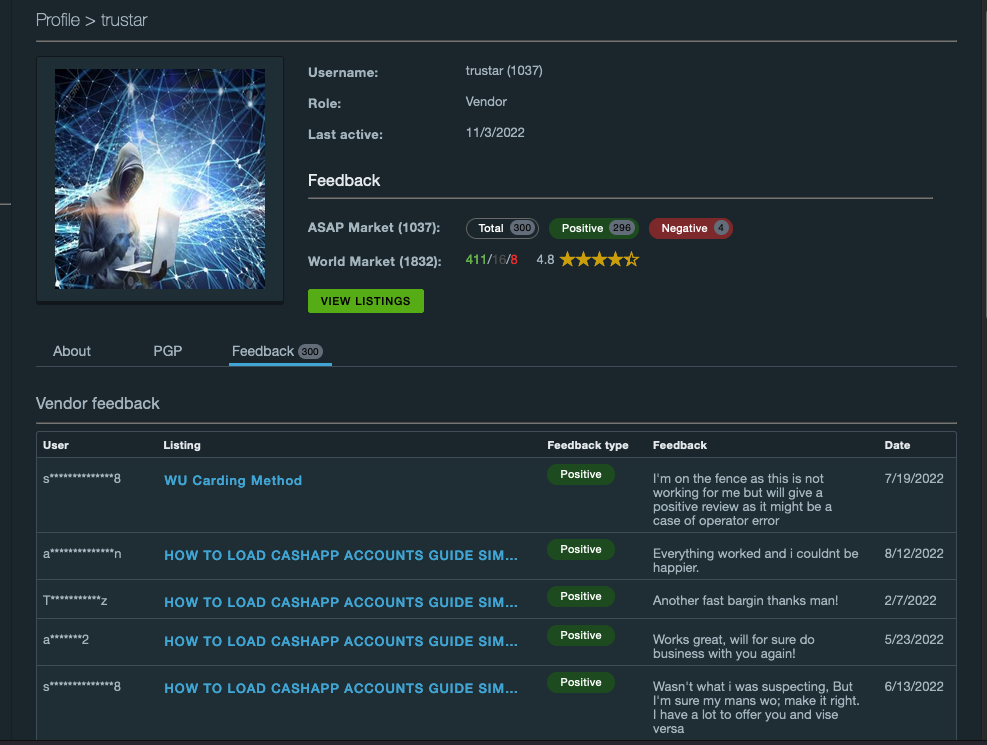
\includegraphics[height=\textheight,width=\textwidth,keepaspectratio]
    {screenshots/seller_feedback_asap_marketplace.png}
    \caption{A shop page in ASAP marketplace.}\label{fig:seller_asap_market}
\end{figure}

\begin{figure}
    \centering
    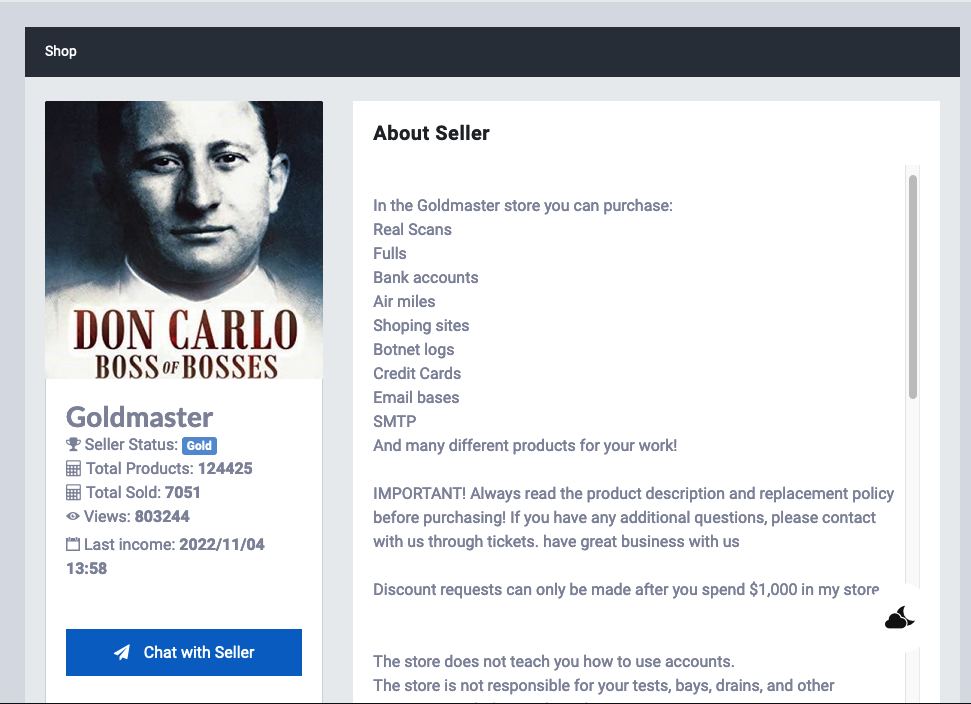
\includegraphics[height=\textheight,width=\textwidth,keepaspectratio]
    {screenshots/seller_page.png}
    \caption{A shop page in Database marketplace.}\label{fig:seller_Database}
\end{figure}
\pagebreak

\section{Results}\label{sec:result}
In this section, I will provide logical explaination and statistical results,
illustrated as figures or tables, to address research questions mentioned in
\autoref{sec:research_questions}.

\subsection{RQ1: What types of stolen information are traded?}
%
As shown in \autoref{fig:type_allocation}, I captured in total 10 product types
based on my own standard. Among all categories, \emph{Personal Data} is the
most active field, contributing \(68,69\%\) of all traded items. \emph{Online Account}
represents the second larges portion \(17,73\%\). The rest of product types ranges
from \(0,36\%\) to \(3,45\%\). Detailed description of each product type is in
\autoref{tab:category_description}.

\begin{table}
    \centering
    \begin{tabular}{|c|c|}
        \hline
        Product type & Description\\
        Personal Data & Full name, date of birth, social security number, home
        address, zip code, driver license, employer info, etc.\\
        Online Account & online account of services such as Netflix, Amazon,
        Venmo, Booking.com, etc.\\
        Bank Account & Username/password of online bank accounts, and credential
        information linked to bank accounts.\\
        Credit Card & card holder name, \acrshort{cvv}, full name, address,
        bank name, card type.\\
        Passport & Real photos and scan of passports.\\
        Email & Emails leaked through data breaches.\\
        Lookup Service & \acrshort{ssn}/\acrshort{dob}/\acrshort{mmn}/\acrshort{dl}
        /\acrshort{cs} lookup service.\\
        Bank Identity Number & \acrshort{bin} is the first 6 digits of the credit card (with
        the help of this information you will understand what credit cards you need to
        work with 3-D Secure VBV) 3-D Secure VBV is a protocol that is used as an
        additional layer of security for online credit and debit cards, two-factor
        user authentication.\\
        Remote Desktop Protocol & The protocol provides user graphical interface to connect
        to other computers over the network connection~\cite{web:rdp_wiki}.\\
        Other & Tutorials, digital document templates, document forms, domains, etc.\\
        \hline
    \end{tabular}
    \caption{Description of product types.}\label{tab:category_description}
\end{table}

\subsection{RQ2: What are the prices for different product types?}
%
There are 6/10 categories, providing more than 90\% of all traded items, 
recording the arithmetic mean price less than 20 USD\@. Furthermore, it supports
the numerical result of 15,87 USD (\autoref{tab:dataset_stat}), the average
price of the whole dataset. The average price of compromised emails is 158,5 USD,
the highest number over all product types. About 10\% of them are email leads,
being recorded 939,19 USD of average price. That explains why the average price
of email type is significantly higher than the overall mean price. In constrast,
products in \emph{Personal Data} field is observed the lowest average price ---
8,71 USD\@. It can be infered that regular Internet users are able to afford
others' indentity information at unexpected-low cost.

\begin{figure}
    \centering
    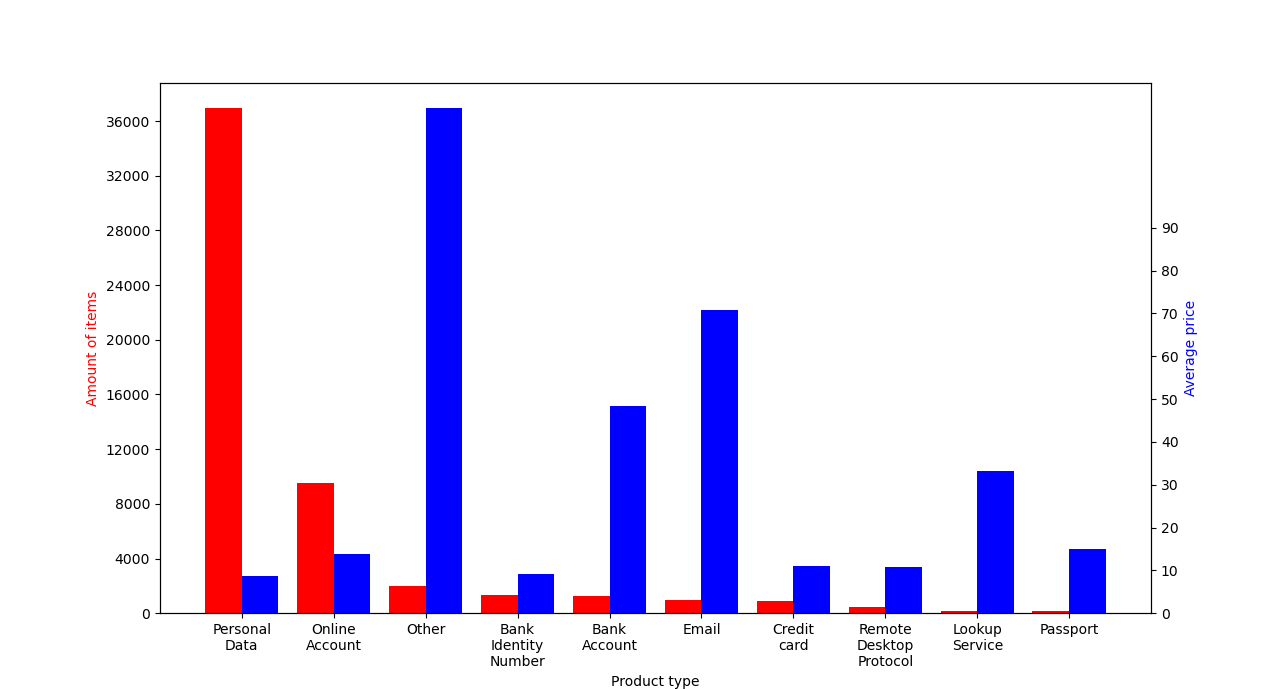
\includegraphics[height=\textheight,width=\textwidth,keepaspectratio]
    {plots/cate_prods_avg_price.png}
    \caption{Number of products and average price over product types.}
    \label{fig:cate_avg_prod}
\end{figure}

\subsection{RQ3: Where the stolen information is from?}
%
The traded information is mainly from data breaches at high-traffic web
services. In \autoref{tab:data_breaches}, I collected a list of major data breaches.
A potential dataset from the breach is traded in Database marketplace, as shown
in \autoref{fig:best_buy_breach}. Information leaked through data breaches can be
email address, password, or more sensitive data, including banking account,
\acrshort{ssn}, and identity information. Moreover, exposed data can be utilized
in attacking campaigns that either trick victims to provide more their own personal
data or unauthorizedly access others account owned by the same user.

\begin{table}
    \begin{tabular}{|c|c|c|}
        \hline
        Name of service & Year & Number of victims\\
        Capital One & 2019 & 100 million Americans and 6 million Canadians\\
        Yahoo & 2013, 2014 & 3 billion, 500 million\\
        Marriott International & 2018 & 500 million\\
        First American Financial & 2019 & 885 million\\
        Facebook & 2019 & 540 million\\
        [24]7.ai --- Bestbuy, Sears, Delta & 2017 & Sears: 100000, Delta: several hundred
        thoudsands, Bestbuy: ``a small fraction of online customers'' 
    \end{tabular}
    \caption{List of major data breaches~\cite{web:best_buy_breach,web:capital_one_breach,
    web:personal_info_darkweb}.}\label{tab:data_breaches}
\end{table}

\begin{figure}
    \centering
    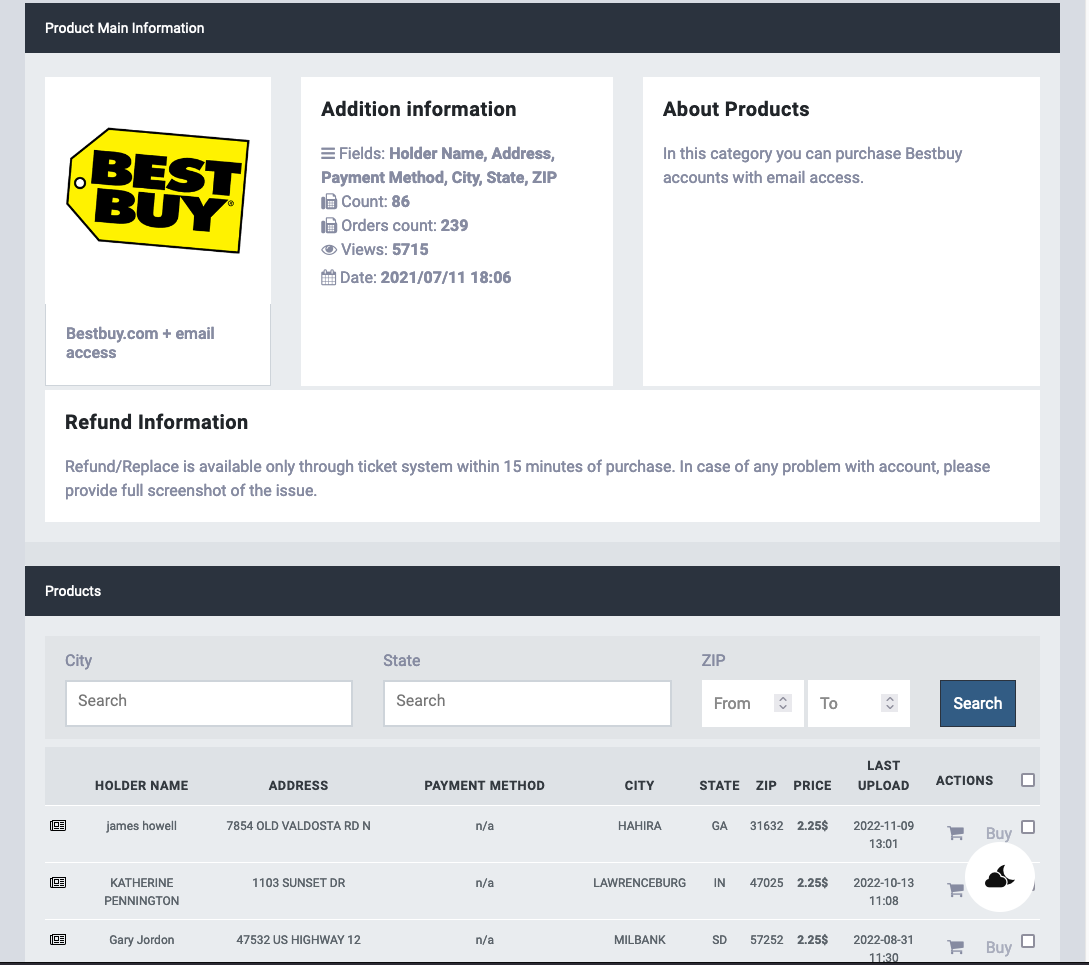
\includegraphics[width=\textwidth,height=\textheight,keepaspectratio]
    {screenshots/best_buy_info.png}
    \caption{Leaked information of Bestbuy's customer.}\label{fig:best_buy_breach}
\end{figure}

\subsection{RQ4: What we can learn about the sellers?}
%
In general, there are two types of sellers, a store sells a large amount of low-cost
items and the one provides a small amount of expensive products (\autoref{fig:avg_prods_seller}).
In anonymous marketplaces, personal contacts of the vendors are unavailable.
To become a seller, a visitor has to provide a list of his/her available products.
Moreover, feedbacks from other anonymous forums and markeplaces need to be sent
to administrators of Database market to prove that the applicant is a valid merchant.

\begin{figure}
    \centering
    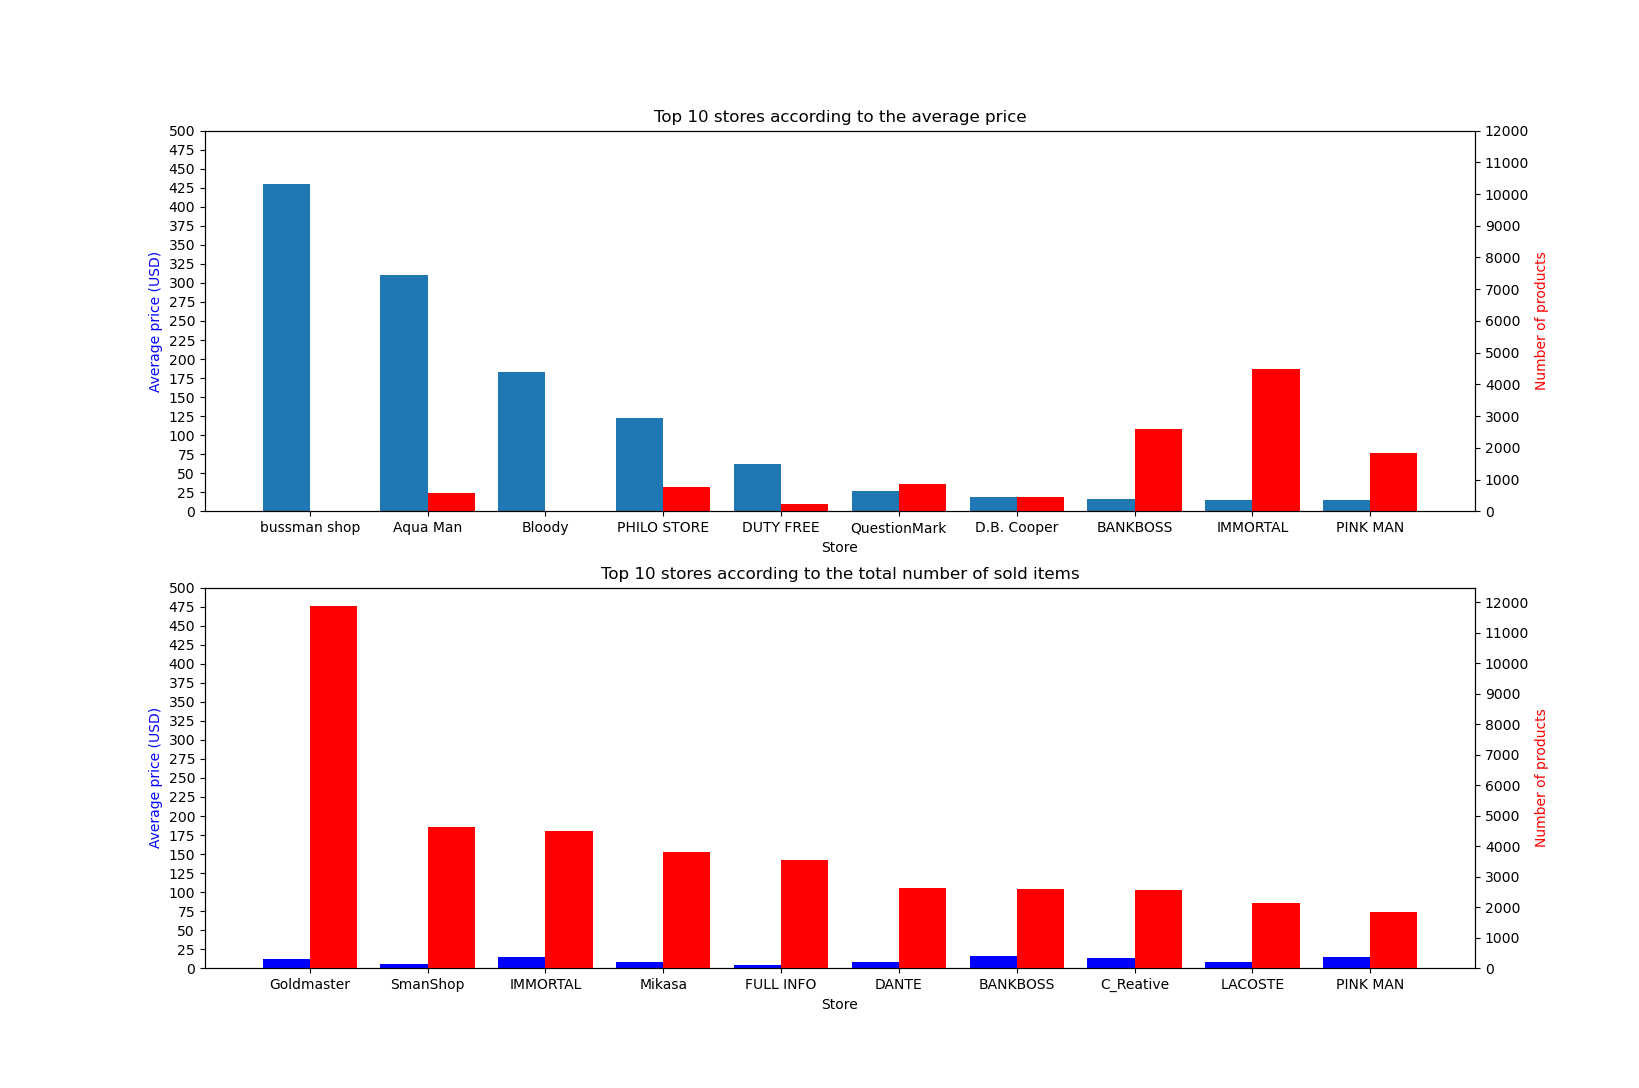
\includegraphics[width=\textwidth,height=\textheight,keepaspectratio]
    {plots/top_avg_price_num_prods_seller.png}
    \caption{Top sellers sorted based on the average price and total number
    of traded products.}\label{fig:avg_prods_seller}
\end{figure}
\pagebreak

\section{Conclusions}\label{sec:conclusion}
It is recorded that there are more than 53815 items was traded in the period
11/2021--06/2022, and more than half of them --- 68,69\% --- are personal data
, including full name, \acrlong{dob}, \acrlong{ssn}, \acrlong{dl}, \acrlong{cs},
etc. The second
most traded product type is username and password pair for accessing online
services of banking, entertaining, and shopping. Both aforementioned product
categories are traded at unexpectedly low cost, less than 15 USD for an entry or
a set of data. The cheapest item are sold at only 0.2 USD for an entry of personal
data (\emph{full name + date of birth + social security number}). Those personal
information is highly possible that are stolen from major data breaches. Through
those data breaches, an attacker gains a set of intial dataset of credential data
that is utilized to trick people trustfully provide more their sensitive data or
access to their online accounts of essential services such as banking or social
security. The consequences of identity theft have been documented thoroughly.
For example, identity thieves can use stolen \acrshort{ssn}s to apply for more
credit and then do not pay the bills, damaging credit of compromised identities~\cite{web:identity_theft}.
As there is a increasing number of data breaches over time, resulting the personal
data is traded at low-cost and highly available, the negative consequences can impact
a wider range of people.

Besides stolen sensitive data, Database marketplace also provides illicit services
such as faking passports, and other identity documents. Ranging from 20 to 1200 USD,
you can order a customized identity document. In addition to an affordable price range,
those services are coveniently traded through the Tor-based marketplace, Database in
this study. The marketplace supports functions, including chatting with sellers, 
searching keywords, and refunding orders, as the normal marketplace, e.g, Ebay.

In conclusion, Database marketplace a wide range of affordable products which
can be utilized to do illegal activities. Moreover, these products are highly
available and sold at reasonable prices; thus, an increasing number of criminal
acts related to identity theft, bank withdrawing, or credit abusing has been
observed. Those acts have rocketing impact on victims, not only financial but
also mental health.

\pagebreak

\printbibliography{}
\pagebreak

\appendix
\section{Tables of statistic results of stores and item categories}
\begin{filecontents*}[overwrite]{category_stat.csv}
    Category,Number of products,Average price
    Personal Data,36963,8.71
    Online Account,9539,13.88
    Other,1855,68.54
    Bank Identity Number,1368,9.24
    Bank Account,1266,48.49
    Email,1102,158.50
    Credit card,892,11.00
    Remote Desktop Protocol,446,10.85
    Lookup Service,192,33.30
    Passport,192,14.94
\end{filecontents*}

\begin{filecontents*}[overwrite]{store_stat.csv}
    seller,num of prods,type range,min price,max price,avg price,med price
    Goldmaster,11882,4,1.0,2500.0,12.24,3.0
    SmanShop,4614,1,1.0,35.0,5.24,5.0
    JOKER,1700,5,1.0,500.0,13.72,6.0
    Goodnik7,1505,2,1.0,15.0,5.06,7.0
    Mikasa,3811,5,1.0,200.0,8.22,5.0
    PINK MAN,1850,4,1.0,1000.0,14.35,5.0
    DANTE,2644,3,0.5,490.0,8.38,3.0
    Dark Shop,1444,6,1.0,350.0,6.5,1.0
    LACOSTE,2124,4,1.0,500.0,8.23,8.0
    IMMORTAL,4484,7,0.5,1600.0,14.48,7.0
    Radikula Store,776,4,0.5,350.0,13.41,6.0
    C\_Reative,2569,5,1.0,2000.0,13.13,10.0
    Hurricane,1254,6,0.5,700.0,7.83,4.0
    FULL INFO,3550,2,1.0,80.0,3.74,4.0
    D.B. Cooper,441,3,1.0,300.0,19.04,5.0
    QuestionMark,857,3,1.0,650.0,26.45,5.0
    NERO,1229,4,1.0,1000.0,12.81,1.0
    Carsh,92,2,3.5,75.0,10.14,3.5
    makataO,833,2,1.0,1000.0,10.51,1.0
    The Best Banks,641,5,0.5,80.0,11.12,10.0
    bussman shop,9,1,80.0,1200.0,430.0,150.0
    DUTY FREE,229,5,2.0,250.0,62.47,10.0
    PHILO STORE,770,7,1.0,550.0,122.22,18.0
    Ninja Secret's,421,4,7.0,50.0,8.8,7.0
    BANKBOSS,2583,6,1.0,670.0,16.64,10.0
    Aqua Man,590,5,0.2,1900.0,310.68,15.0
    PROMETHEUS,315,3,1.0,60.0,6.62,1.0
    BestLink,588,4,3.0,250.0,10.21,6.0
    Spamking,7,1,7.0,7.0,7.0,7.0
    Bloody,3,1,150.0,200.0,183.33,200.0
\end{filecontents*}

\begin{table*}[h!]
    \centering
    \csvreader[tabular =|c|c|c|c|,
    table head=\hline Category & Amount of products & Average price\\\hline,
    late after line=\\\hline]%
    {category_stat.csv}{Category=\cate, Number of products=\amount, Average price=\avg}%
    {\cate\ & \amount\ & \avg}%
    \caption{Amount of products and average price of product categories. The currency of price is USD.}
    \label{tab:category_stat}
\end{table*}

\begin{landscape}
    \begin{table*}[]
        \centering
        \csvreader[tabular =|c|c|c|c|c|c|c|,
        table head=\hline Store & Amount of products & Range of types & Min price &
        Max price & Average pirce & Median price\\\hline,
        late after line=\\\hline]%
        {store_stat.csv}{seller=\a,num of prods=\b,type range=\c,
        min price=\d,max price=\e,avg price=\f,med price=\g}%
        {\a\ & \b\ & \c\ & \d\ & \e\ & \f\ & \g}%
        \caption{Statistical results of stores. The currency of price is USD.}
        \label{tab:store_stat}
    \end{table*}
\end{landscape}


\section{Screenshots of Database marketplace}
\begin{figure}
    \centering
    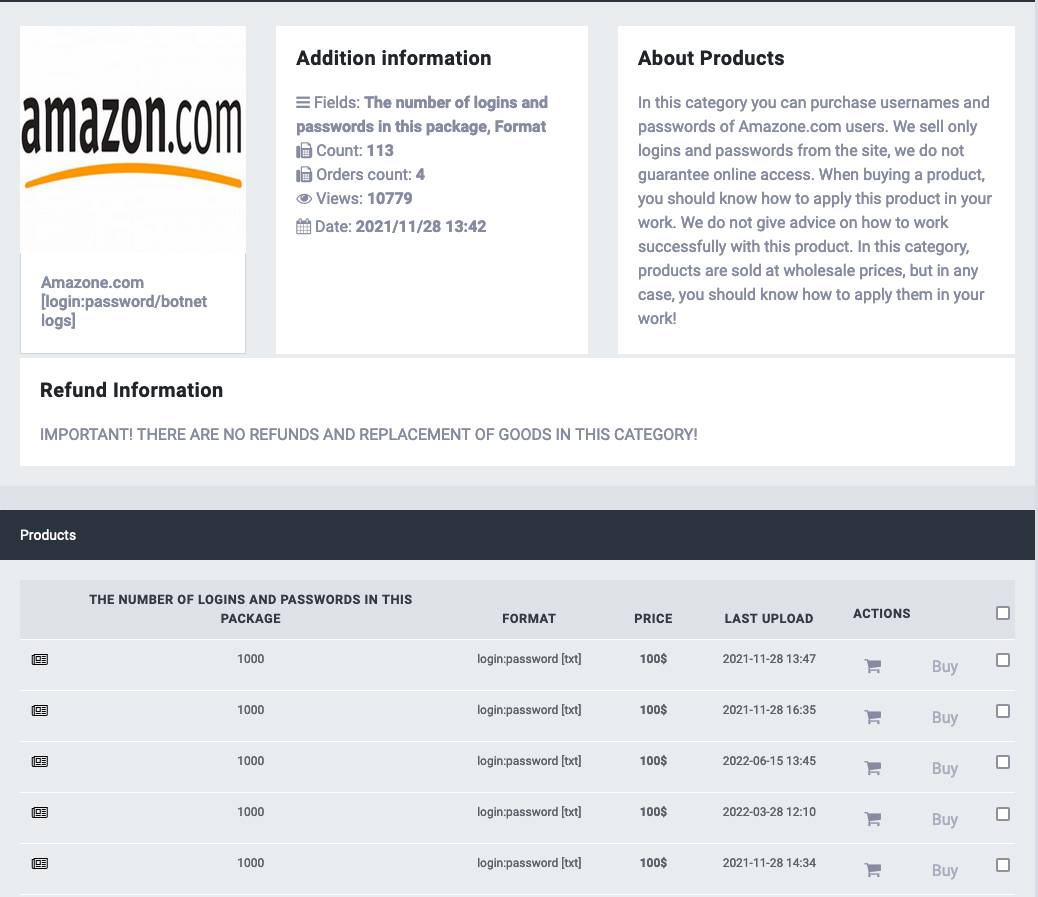
\includegraphics[height=\textheight,width=\textwidth,keepaspectratio]
    {screenshots/amazon_acc_bulk.png}
    \caption{Leaked Amazon accounts}\label{fig:amazon}
\end{figure}

\begin{figure}
    \centering
    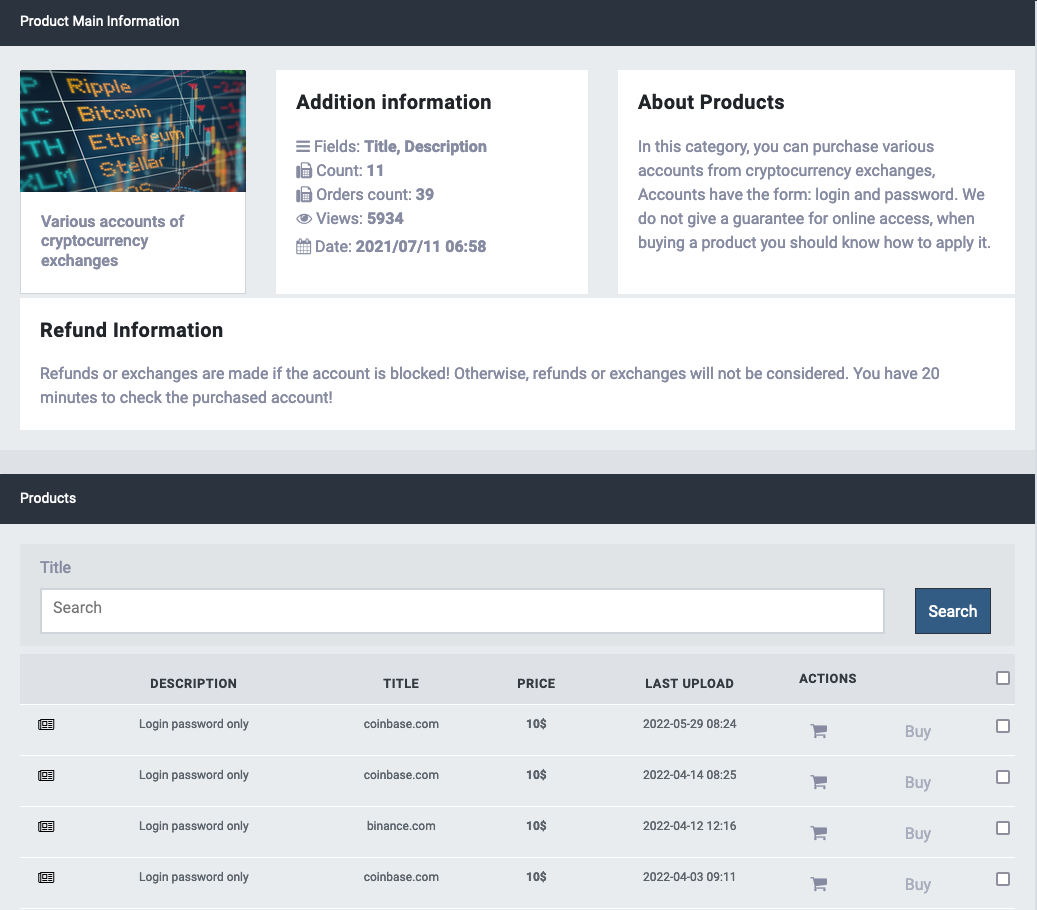
\includegraphics[height=\textheight,width=\textwidth,keepaspectratio]
    {screenshots/crypto_acc.png}
    \caption{Leaked Cryptocurrency exchange accounts}\label{fig:crypto_exchange}
\end{figure}

\begin{figure}
    \centering
    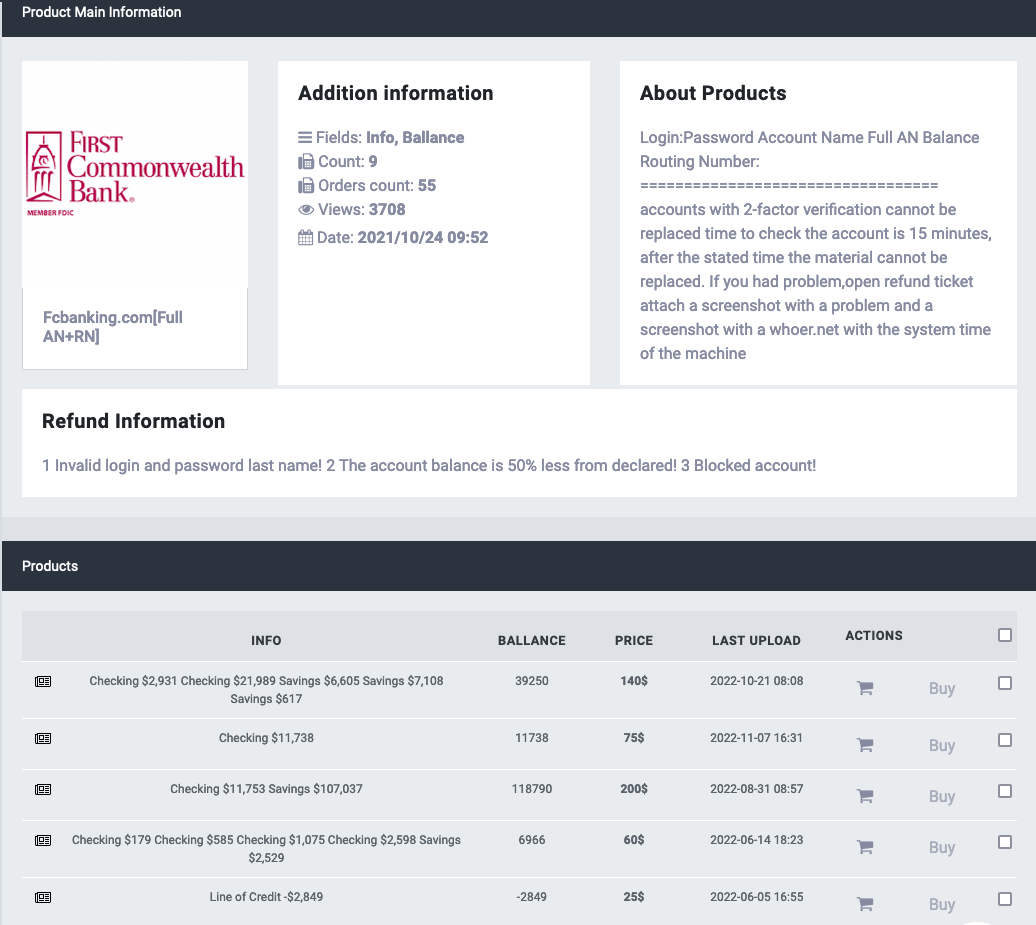
\includegraphics[height=\textheight,width=\textwidth,keepaspectratio]
    {screenshots/bank_acc.png}
    \caption{Leaked bank accounts}\label{fig:leaked_bank}
\end{figure}

\begin{figure}
    \centering
    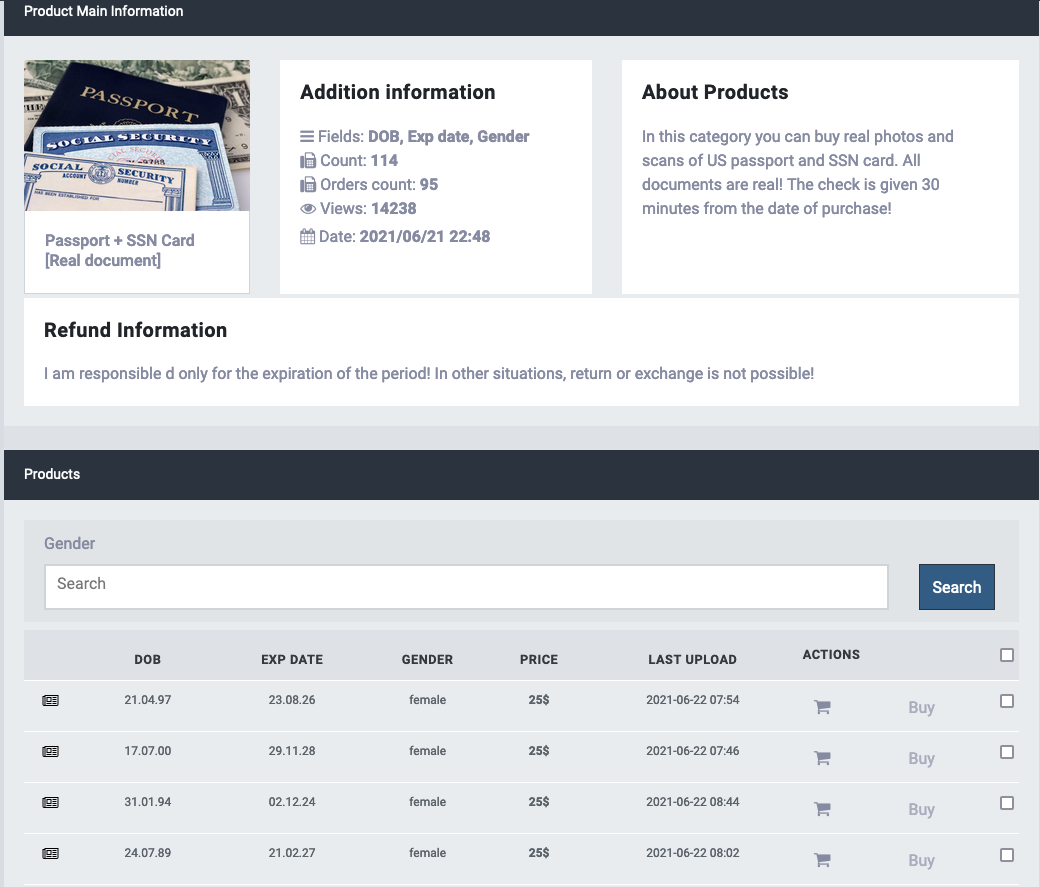
\includegraphics[height=\textheight,width=\textwidth,keepaspectratio]
    {screenshots/leaked_scan_passport.png}
    \caption{Leaked passports}\label{fig:passport}
\end{figure}

\end{document}